\documentclass{beamer}

\usepackage{pgf}
\usepackage{calc}
\usepackage{amsmath}
\usepackage{amssymb}
\usepackage{amsthm}
\usepackage[latin1]{inputenc}
\usepackage{beamerthemesplit}
\usepackage{alltt}
\usepackage{graphics}

\usetheme{Cea}

\newcommand{\rouge}[1]{{\color{red}#1}}
\newcommand{\bleu}[1]{{\color{blue}#1}}
\newcommand{\monvert}[1]{{\color{green}#1}}
\newcommand{\motcle}[1]{{\color{blue}#1}}
\newcommand{\ocamlgraph}{\textsf{OcamlGraph}}
\newcommand{\fleche}{\ensuremath{\rightarrow}}
\newcommand{\vara}{\ensuremath{\alpha}}
\newcommand{\varb}{\ensuremath{\beta}}

\newcommand{\excode}[1]{\monvert{\texttt{#1}}}
\newcommand{\present}{{\monvert{\large\boldmath $\surd$}}}
\newcommand{\absent}{\rouge{\large\boldmath $\oslash$}}

\newcommand{\oemph}[1]{\textcolor{orange}{#1}}
\let\emph\oemph

\title{Designing a Generic Graph Library using ML Functors}

%%%%%%%%%%%%%%%%%%%%%%%%%%%%%%%%%%%%%%%%%%%%%%%%%%%%%%%%%%%%%%%%%%%%%%%%%%%%%%%

\begin{document}

\setbeamertemplate{navigation symbols}{}

%%%%%%%%%%%%%%%%%%%%%%%%%%%%%%%%%%%%%%%%%%%%%%%%%%%%%%%%%%%%%%%%%%%%%%%%%%%%%%%

\begin{frame}
  \begin{center}
    \textcolor{orange}{\Large Designing a Generic Graph Library \\[0.7em]
      using ML Funtors}\\[2em]

    \textcolor{blue}{\large Sylvain Conchon, Jean-Christophe Filli�tre}
    \\[0.7em]
    \textcolor{green}{\large LRI, Paris Sud University}\\[1.4em]
    \textcolor{blue}{\large \textit{Julien Signoles}}\\[0.7em]
    \textcolor{green}{\large CEA LIST, Software Safety Labs}
  \end{center}
\end{frame}

%%%%%%%%%%%%%%%%%%%%%%%%%%%%%%%%%%%%%%%%%%%%%%%%%%%%%%%%%%%%%%%%%%%%%%%%%%%%%%%

%\section[Introduction]{}

\begin{frame}
  \frametitle{OcamlGraph}
  \begin{itemize}
  \item \emph{What is \ocamlgraph}
    \begin{center}
      A  graph library for Ocaml
      
      \bleu{\url{http://www.lri.fr/~filliatr/ocamlgraph}}
    \end{center}
    \pause\vskip10pt
  \item
    \emph{Why \ocamlgraph?}
    \begin{center}
      Before, no graph library for Ocaml.
    \end{center}
    \pause\vskip10pt
  \item \emph{Why \textsl{a talk about} \ocamlgraph?}
    \begin{center}
      Designing a generic graph library is not so easy:
    \end{center}
    \begin{itemize}
    \item How to easily provide many different graph data structures?
    \item How to provide reusable graph algorithms? 
    \end{itemize}
    \begin{center}
      \bleu{Our solution: ML functors.}
    \end{center}
  \end{itemize}
\end{frame}

\begin{frame}
  \frametitle{Outline}
  \begin{itemize}
  \item Graph data structures: interface\vskip15pt
  \item Graph data structures: implementation\vskip15pt
  \item Graph algorithms\vskip15pt
  \item Conclusion
  \end{itemize}
\end{frame}

%%%%%%%%%%%%%%%%%%%%%%%%%%%%%%%%%%%%%%%%%%%%%%%%%%%%%%%%%%%%%%%%%%%%%%%%%%%%%%%

%\section[Interface]{}

\begin{frame}
  \frametitle{Outline}
  \begin{itemize}
  \item Graph data structures: interface\vskip15pt
  \item \textcolor{black!30}{Graph data structures: implementation\vskip15pt
  \item Graph algorithms\vskip15pt
  \item Conclusion}
  \end{itemize}
\end{frame}

\begin{frame}[containsverbatim]
  \frametitle{Interfaces}
  \emph{Common interface for all graphs:}
  \begin{alltt}
    module type \bleu{G} = sig ... end    
  \end{alltt}
  \emph{Interface for persistent graphs:}
  \begin{alltt}
    module type \bleu{P} = sig
      include \bleu{G}
      ...
    end
  \end{alltt}
  \emph{Interface for imperative graphs:}
  \begin{alltt}
    module type \bleu{I} = sig
      include \bleu{G}
      ...
    end
  \end{alltt}
\end{frame}

\begin{frame}[containsverbatim]
  \frametitle{Kinds of graph}
  \begin{center}
    \bleu{What kind of graph do you want to use?}
  \end{center}
  \begin{itemize}
  \item Mutable graph or not?
    \hfill \excode{Imperative} or \excode{Persistent}
    \vskip10pt
  \item Directed or not?
    \hfill \excode{Digraph} or \excode{Graph}
    \vskip10pt
  \item Abstract vertices or not?
    \hfill \excode{Abstract} or \excode{Concrete}
    \vskip10pt
  \item Label on edges or not?
    \hfill \excode{Labeled} (or nothing)
  \end{itemize}
  \begin{center}
    Example: \excode{Imperative.Digraph.AbstractLabeled}\vskip10pt
  \end{center}
\end{frame}

\begin{frame}\frametitle{Components}
  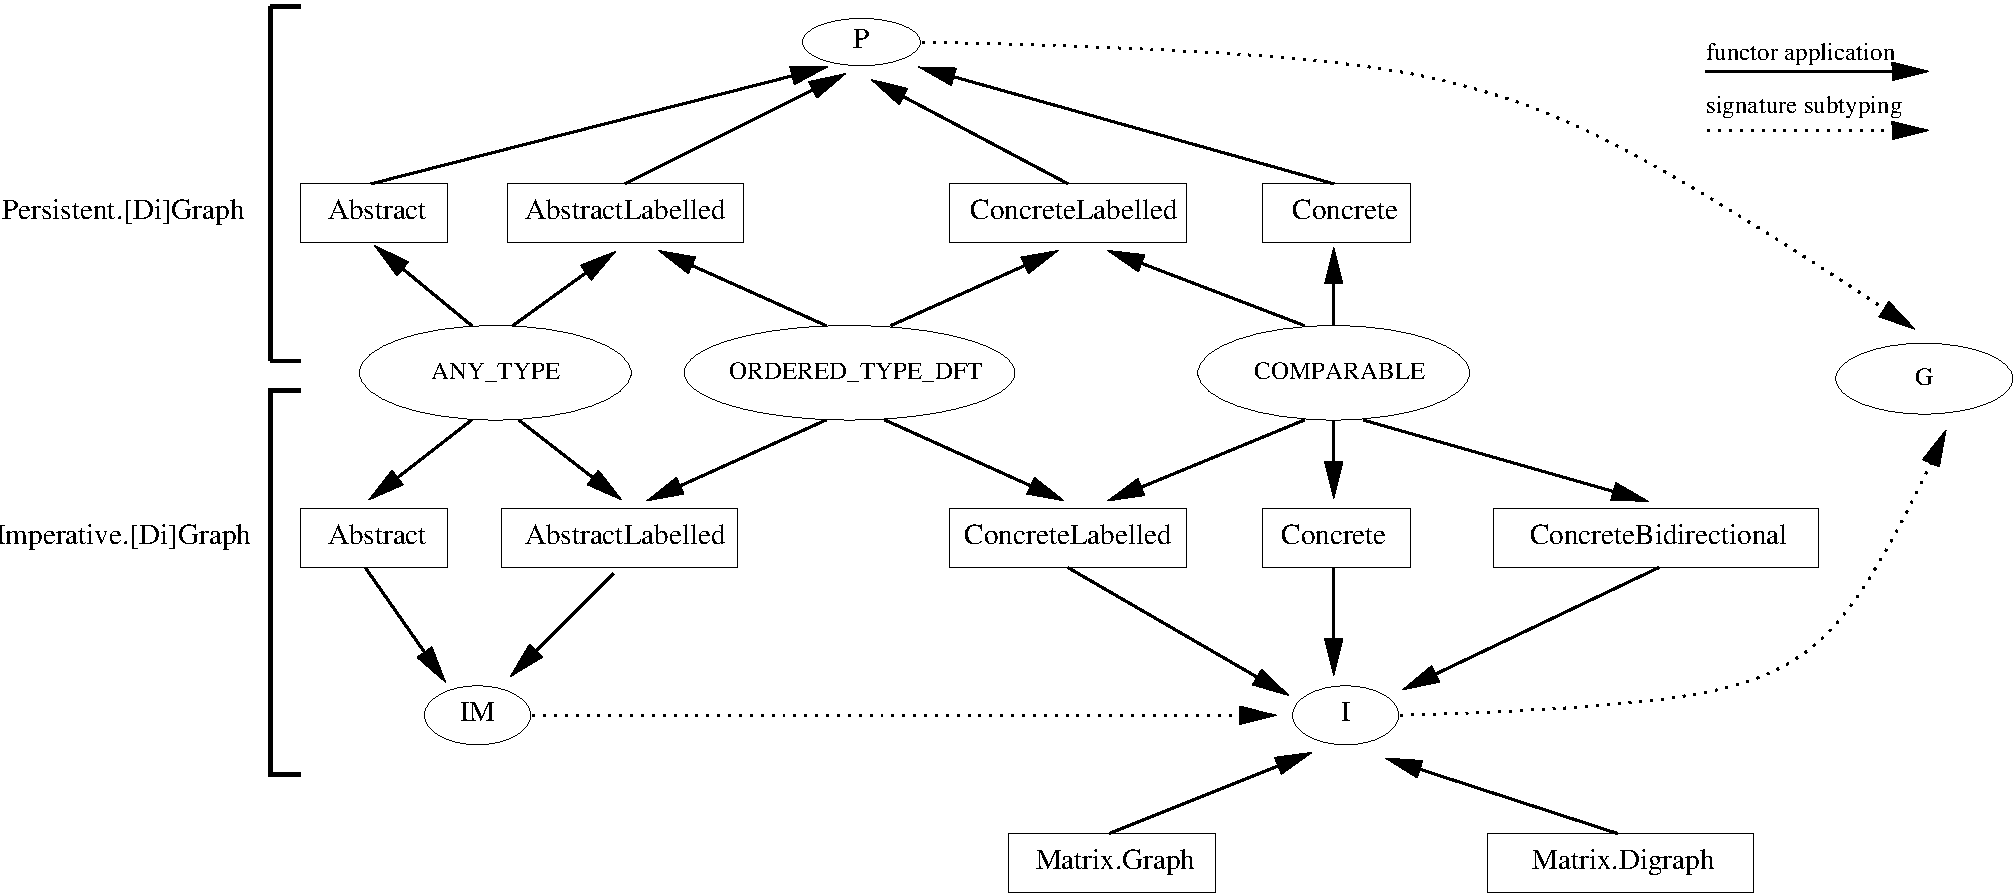
\includegraphics[width=\textwidth]{interface.pdf} 
\vskip-1pt
\begin{itemize}
\item 8 \bleu{persistent}: implemented with \texttt{Map}.
\item 8 \bleu{imperative}: implemented with \texttt{Hashtable}.
\item 3 \bleu{specialized}: adjacency matrices and bidirectional graphs.
\end{itemize}
\vskip-3pt
\begin{center}\emph{All together, 19 data structures}.\end{center}
\end{frame}

%%%%%%%%%%%%%%%%%%%%%%%%%%%%%%%%%%%%%%%%%%%%%%%%%%%%%%%%%%%%%%%%%%%%%%%%%%%%%%%

%\section[Implementation]{}

\begin{frame}
  \frametitle{Outline}
  \begin{itemize}
  \item \textcolor{black!30}{Graph data structures: interface\vskip15pt}
  \item Graph data structures: implementation\vskip15pt
  \item \textcolor{black!30}{Graph algorithms\vskip15pt
  \item Conclusion}
  \end{itemize}
\end{frame}

\begin{frame}
  \frametitle{Providing specialized blocks}
  \begin{center}
    \bleu{How to provide 19 implementations of the same signature without code
    dupplication?}
  \end{center}
  \pause
  \begin{enumerate}
  \item Abstracting the underlying implementation (map or hashtable) by using a
  common signature \excode{HM}. 
  \vskip8pt\pause
  \item Providing specialized blocks as functors parameterized by a \excode{HM}
    implementation and by others operations:
    \vskip1pt
    \begin{itemize}
    \item \excode{Minimal}: common operations to all data structures.
      \vskip6pt
    \item \excode{Labeled}/\excode{Unlabeled}: operations on (un)labeled edges.
      \vskip6pt
    \item \excode{Pred}: operations on predecessors from successors.
      \vskip6pt
    \item \excode{Make\_Abstract}: operations on abstract graphs from a
    concrete version.
    \end{itemize}
  \end{enumerate}
\end{frame}

\begin{frame}[containsverbatim]
  \frametitle{Putting blocks together}
\begin{center}
\excode{Make}: an higher-order functor.
\end{center}
\begin{alltt}
\motcle{module} Make
  (F: \motcle{functor}(X: COMPARABLE) \fleche
      HM \motcle{with type} key = X.t) = 
\motcle{struct}
  \motcle{module} Digraph = \motcle{struct}
    \motcle{module} Concrete(V: COMPARABLE) = \motcle{struct}
      \motcle{include} ConcreteVertex(F)(V)
      \motcle{include} Unlabeled(V)(HM)
      \motcle{include} Minimal(S)(HM)
    \motcle{end}
    ...
\motcle{end}
\end{alltt}
\end{frame}

\begin{frame}[containsverbatim]
  \frametitle{Instantiation and specialisation}
  \begin{alltt}
\motcle{module} P = Make(Make_Map)
\motcle{module} Digraph = struct
  \motcle{module} Concrete (V: COMPARABLE) = \motcle{struct}
    \motcle{include} P.Digraph.Concrete(V)
    \motcle{let} add_vertex g v = 
      \motcle{if} HM.mem v g \motcle{then} g 
      \motcle{else} unsafe_add_vertex g v
    ...
  \motcle{end}
\motcle{end}
\end{alltt}

  \begin{center}
    All together, 19 data structures with 45 operations, i.e.
    
    \emph{855 operations in 1000 lines of code}.
  \end{center}
\end{frame}

%%%%%%%%%%%%%%%%%%%%%%%%%%%%%%%%%%%%%%%%%%%%%%%%%%%%%%%%%%%%%%%%%%%%%%%%%%%%%%%

\begin{frame}
  \frametitle{Outline}
  \begin{itemize}
  \item \textcolor{black!30}{Graph data structures: interface\vskip15pt
  \item Graph data structures: implementation\vskip15pt}
  \item Graph algorithms\vskip15pt
  \item \textcolor{black!30}{Conclusion}
  \end{itemize}
\end{frame}

\begin{frame}
  \frametitle{Generic programming}

  \begin{center}
    Write algorithms independently of the graph implementation.\\[1.2em]
    \emph{Algorithm = functor}\\
    in which parameters only contain the required operations.
  \end{center}

  \pause
  \begin{itemize}
  \item \emph{Use} it on non-\ocamlgraph\ data structures.\vskip8pt
  \item \emph{Implement} it more safely.\vskip8pt
  \item \emph{Extend} the library more easily.\vskip8pt
  \end{itemize}
\end{frame}

\begin{frame}
  \frametitle{Existing algorithms}
  \begin{itemize}
  \item Traversal: 7 DFS, 2 BFS, 2 cycle detections
  \item Building:
    \begin{itemize}
    \item 4 classics (ex. de Bruijn's graph)
    \item 2 randoms (ex. planar graph) 
    \end{itemize}
  \item Dijkstra's shortest path
  \item Strongly connected components
  \item Goldberg's and Ford-Fulkerson's maximal flow.
  \item $k$-coloring
  \item Topological sorting
  \item Kruskal's minimum spanning tree
  \item Misc. operations: transitive closure, complementary, miror,
    neighbourhood, \dots
  \item Interfaces with Graphviz and GML.
\end{itemize}
\end{frame}

\begin{frame}
  \frametitle{Example}
  \begin{center}Flow algorithms\end{center}
\end{frame}

%%%%%%%%%%%%%%%%%%%%%%%%%%%%%%%%%%%%%%%%%%%%%%%%%%%%%%%%%%%%%%%%%%%%%%%%%%%%%%%

%\section[Conclusion]{}

\begin{frame}
  \frametitle{Outline}
  \begin{itemize}
    \item \textcolor{black!30}{Graph data structures: interface\vskip15pt
    \item Graph data structures: implementation\vskip15pt
    \item Graph algorithms\vskip15pt}
  \item Conclusion
  \end{itemize}
\end{frame}

\begin{frame}
  \frametitle{Comparison}
  \begin{tabular}{|l||c|c|c|c|c|}
    \hline
     Library & Language     &P/I& Genericity & Data struct. \\\hline\hline
     GTL & C++     & I & \absent  & 1  \\\hline
     LEDA & C++    & I & \absent  & 2  \\\hline
     BGL & C++     & I & \present & 2  \\\hline
     JDSL & Java   & I & \present & 1  \\\hline
     FGL & Haskell & P & \absent  & 1  \\\hline
     MLRisc & SML  & I & \absent  & 1  \\\hline
%     Baire & Ocaml &P/I& ---      & 8  \\\hline
     \emph{\ocamlgraph}& Ocaml &P/I& \present & \emph{19} \\\hline
  \end{tabular}
\end{frame}

\begin{frame}
  \frametitle{Numbers}
  \begin{itemize}
  \item \ocamlgraph, that is:\vskip2pt
    \begin{itemize}
    \item $\approx$ 7000 lines of code ($\approx$ 2000 lines of contributions)
      \vskip7pt
    \item 9 men-weeks of works
    \end{itemize}
    \begin{center}
      \emph{Only possible thanks to ML functors.}
    \end{center}\vskip10pt
    \pause
  \item Benchmarks (imperative abstract graphs):\vskip2pt
    \begin{itemize}
    \item create 100 000 edges per second\vskip7pt
    \item visit between 500 000 and 1 million edges per second
    \end{itemize}
    \begin{center}
      \emph{Reasonably efficient.}
    \end{center}
  \end{itemize}
\end{frame}

%%%%%%%%%%%%%%%%%%%%%%%%%%%%%%%%%%%%%%%%%%%%%%%%%%%%%%%%%%%%%%%%%%%%%%%%%%%%%%%

\end{document}
    
